\section{Cosmic rays}
\label{sec:introduction}
Cosmic radiation is made of particles coming from the outer space and can be divided into primary and secondary cosmic rays.

\emph{Primary cosmic rays} consist of particles accelerated at astrophysical sources. Thus electrons,
protons and helium are primaries, as well as carbon, oxygen, iron and other nuclei synthesized in stars \cite{PDG}.
The energy spectrum of primary cosmic rays is rather well known and it is shown in Figure \ref{CRSpectrum}. It extends up to $\SI{e20}{eV}$, 12 orders of magnitude on the energy scale and $32$ orders of magnitude on the flux scale. 
\begin{figure}[!h]
	\centering
	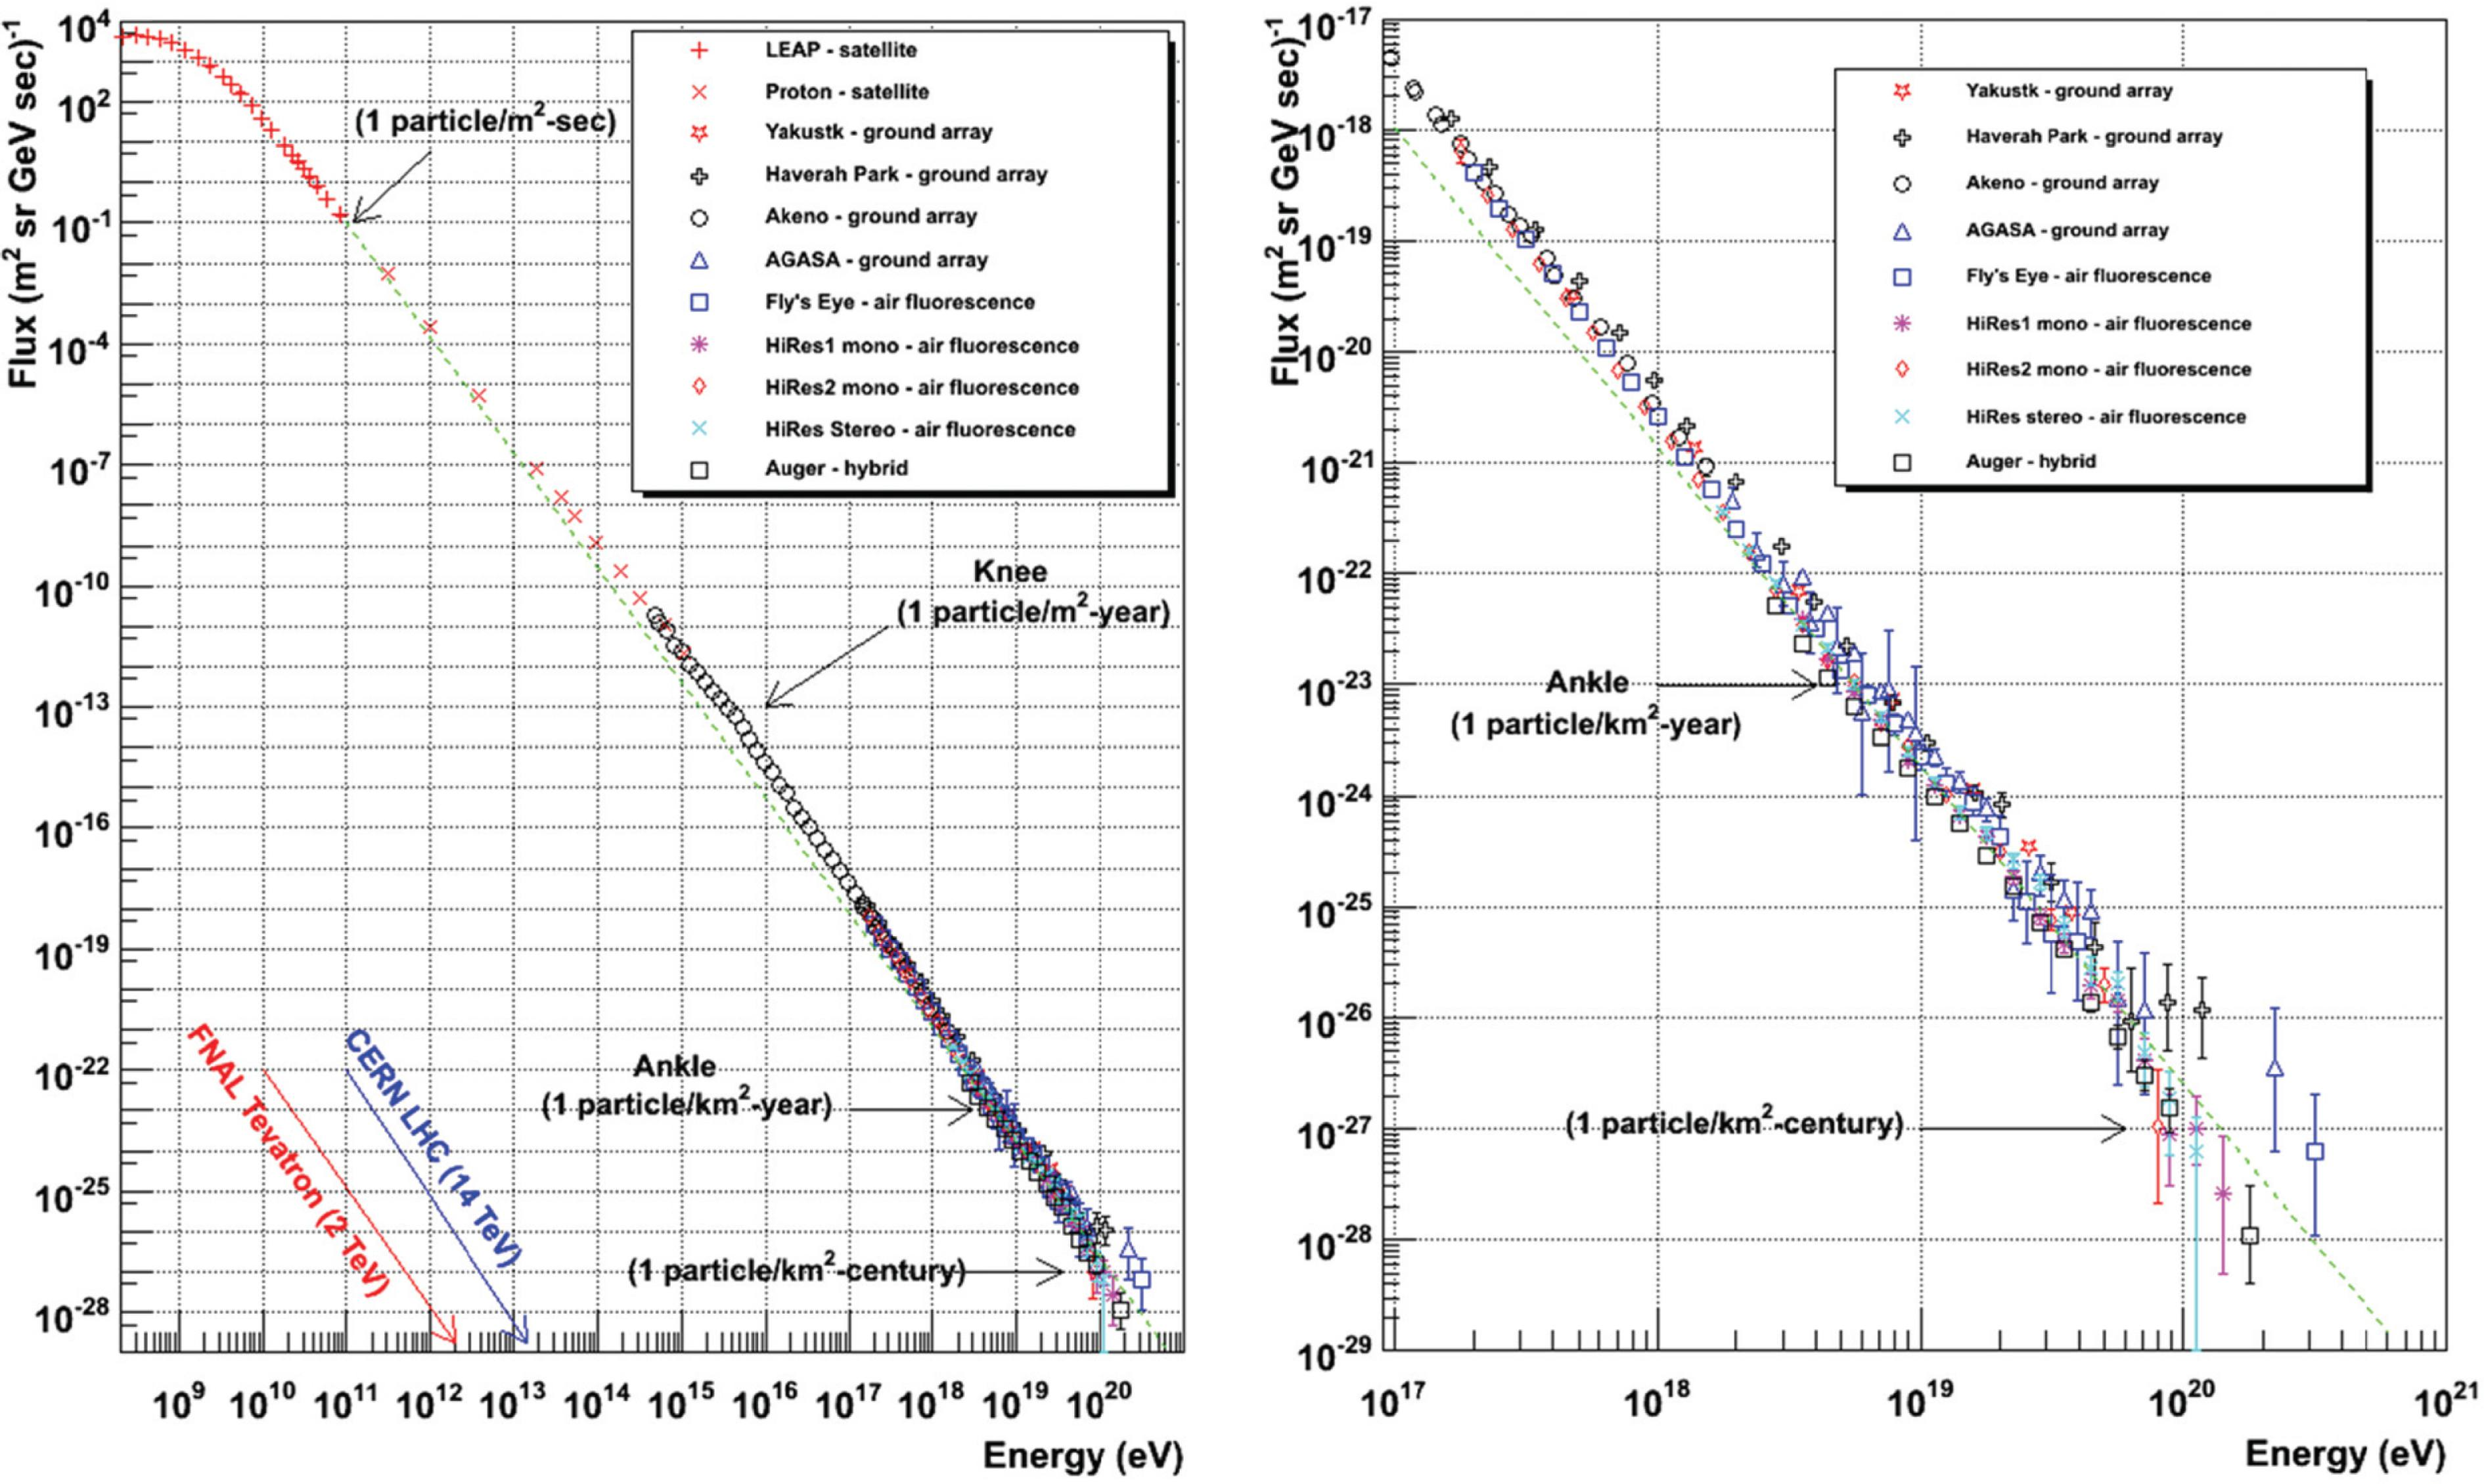
\includegraphics[scale=0.09]{CR_spectrum} 
	
	\caption{Primary cosmic rays flux as a function of the energy [\si{eV}]. To make a comparison, notice that the highest-energy accelerator LHC has a centre of mass energy $\sqrt s = \SI{14}{TeV}$ against $\SI{e20}{eV}$ of maximum energy of cosmic rays. On the other hand at these extreme energies the flux is very low, tipically 1 particle $\si{km^{-2}}$ $\textrm{century}^{-1}$.} \label{CRSpectrum}
\end{figure}

Experimental observations indicate that the differential energy spectrum for primary cosmic rays can be well represented by power-law distributions of the form

\begin{equation}
\frac{\dd N}{\dd E} = k E^{- \gamma}
\end{equation}
where $\gamma$ is the spectral index.
Prominent features in the spectrum are the changes in the slope known as the \emph{knee} at $\SI{e15}{eV}$ and the \emph{ankle} at $\SI{e18}{eV}$ \cite{Longair}.
The spectral index is $\gamma = 2.7$ for energies below the energy of the knee, while for higher energies it changes approximately from $2.7$ to $3$ \cite{Longair}.

\emph{Secondaries} are produced by the interactions of the primaries with the upper Earth's atmosphere\footnote{When discussing the astrophysical origin of cosmic rays, 'secondaries' are those particles produced in interaction of the primaries with the ISM (InterStellar Medium). Nuclei such as lithium, beryllium, and boron are secondaries \cite{PDG}.}.
When primary particles penetrate the atmosphere they interact strongly with air nuclei giving rise to a \emph{hadronic shower} in which pions ($\pi^{\pm}, \pi^0$) are mainly produced, less frequently kaons ($K^{\pm}, K^0$) and even more rarely other hadrons.
Since these particles are unstable they decay into lighter ones, in particular charged kaons and pions decay principally according to the following decay channels 

\begin{equation}
K^+\rightarrow \mu^+ + \nu_{\mu} \qquad
K^-\rightarrow \mu^- + \overline \nu_{\mu} \qquad \tau = \SI{26.03}{ns} \quad \cite{PDG}
\end{equation}

\begin{equation}
\pi^+\rightarrow \mu^+ + \nu_{\mu} \qquad
\pi^-\rightarrow \mu^- + \overline \nu_{\mu} \qquad \tau = \SI{12.38}{ns} \quad \cite{PDG}
\end{equation}
with lifetimes of order $\mathcal{O} (\si{ns})$ and with the production of muons, antimuons and their neutrinos. 
Hadronic collisions produce not only charged pions but also $\pi^0$. The latter decay quickly producing photons ($\pi^0 \rightarrow \gamma \gamma$) which give origin to an \emph{electromagnetic shower}. In fact high-energy photons interact with the nuclei producing an electron-positron pair ($\gamma + N \rightarrow e^+ + e^- + N$) and these leptons in turn can produce photons by bremsstrahlung and so on.

The majority of the decay products cannot reach the Earth's surface since they have a too short lifetime (and not enough energy).
Nevertheless, most of the muons and neutrinos produced by charged pions decay can easily reach the ground due to relativistic effects. 
Therefore muons are the most numerous charged particles
detected at sea level (see Figure \ref{secondary_composition}).
\begin{figure}[!h]
	\centering
	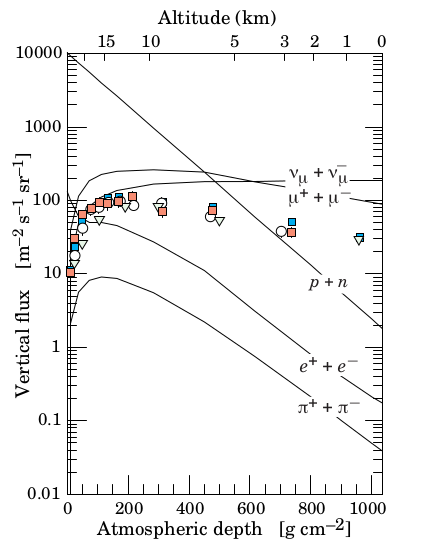
\includegraphics[scale=0.45]{vert_flux} 
	\caption{Vertical fluxes of cosmic rays in the atmosphere with $E > \SI{1}{GeV}$ estimated from nucleon flux. The points show measurements of negative muons with $E_{\mu} > \SI{1}{GeV}$.} \label{secondary_composition}
\end{figure}

Most muons are produced high in the upper atmosphere (typically at $\SI{15}{km}$ altitude) and before reaching the ground they lose about $\SI{2}{GeV}$ due to ionization. Their energy and angular distribution
reflect a convolution of the production spectrum, energy loss in
the atmosphere and decay. 
For example $\SI{2.4}{GeV}$ muons would have a decay length of $\SI{15}{km}$, which is reduced to $\SI{8.7}{km}$ by energy loss.
The mean energy of muons at the ground is $\sim \SI{4}{GeV}$ \cite{PDG}.
%The energy spectrum is almost flat below $\SI{1}{GeV}$, steepens gradually to reflect the primary spectrum in the range 10-100 $\si{GeV}$ and it steepens further at higher energies, since pions with energies greater than the critical energy $\epsilon_{\pi} = \SI{115}{GeV}$ tend to interact in the atmosphere before their decay \cite{PDG}.
%Asymptotically ($E_{\mu} \gg \SI{1}{TeV}$),
%the energy spectrum of atmospheric muons is one power steeper
%than the primary spectrum.\\ 
The flux of vertical muons above $\SI{1}{GeV/c}$ at sea level is $ I_0 \approx 70 \si{m^{-2}} \si{s^{-1}} \si{sr^{-1}}$, which for horizontal detectors is more familiar as

\begin{equation}
\label{mu-rate}
I_0 \approx 1 \si{cm^{-2}} \si{min^{-1}}  \, \cite{PDG} .
\end{equation}

The \emph{muon angular distribution} at the ground as a function of the zenith angle $\theta$ is
\begin{equation} \label{dist}
\frac{\dd N}{\dd \Omega \dd A \dd t} \approx I_0 \cos^2 \theta
\end{equation}
and it is characteristic for muons with $E_{\mu} \sim \SI{3}{GeV}$\footnote{At low energies the angular distribution becomes increasingly steep, while at high energies it flattens, approaching a $\sec \theta$ distribution for $E_{\mu} \gg \epsilon_{\pi} = \SI{115}{GeV}$ and $\theta < \ang{70}$ \cite{PDG}.} \cite{PDG}.
\begin{figure}[!h] 
	\centering
	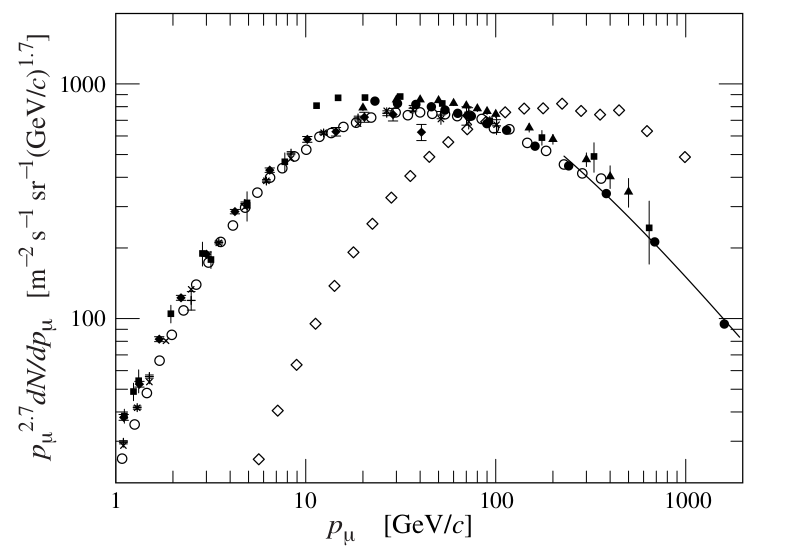
\includegraphics[scale=0.32]{energy_spect} 
	\caption{Spectrum of muons at $\theta = \ang{0}$ ($\blacklozenge , \blacksquare , \blacktriangledown , \blacktriangle , \times , + , \circ, \bullet$) and  $\theta = \ang{75} (\Diamond) $ \cite{PDG}.} \label{energy_spect}
\end{figure}

Figure \ref{energy_spect} shows the muon energy spectrum at sea level for two angles: at large angles the low energy ones decay before reaching the surface, moreover high energy pions decay before they interact, thus the average muon energy increases.

Another important feature of cosmic muons is their measured \emph{charge asymmetry}, which is shown in Figure \ref{muon_asimmetry}. The muon charge ratio $\mu^+ / \mu^-$ reflects either the excess of $\pi^+$ over  $\pi^-$ and
$K^+$ over  $K^-$ in the forward fragmentation region of proton initiated
interactions or the fact that there are more free and bound
protons than free and bound neutrons in the primary spectrum \cite{PDG}. 

\begin{figure}[!h]
	\centering
	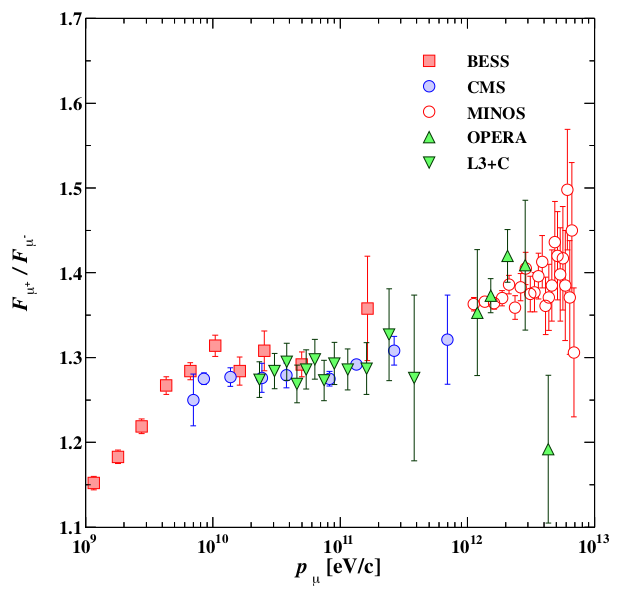
\includegraphics[scale=0.32]{muon_asimmetry} 
	\caption{Muon charge ratio $\mu^+ / \mu^-$ as a function of the muon momentum [\si{eV / c}]. The increase with energy reflects the growing importance of kaons in the $\si{TeV}$ range and it indicates a significant contribution of associated production by cosmic-ray protons ($p \rightarrow \Lambda + K^+ $) \cite{PDG}.} \label{muon_asimmetry}
\end{figure}


\section{Free muon decay}

Muons are unstable particles which decay into electrons with the emission of electron antineutrinos and muon neutrinos\footnote{Positive muons decay in their charged-conjugated final state particles.} according to

\begin{equation} \label{muon decay}
\mu^- \rightarrow e^- + \bar \nu_{e} + \nu_{\mu} \qquad \mu^+ \rightarrow e^+ + \nu_{e} + \bar \nu_{\mu} . 
\end{equation}

The free decay process is described by the Feynman diagram shown in Figure \ref{feynman}.
\begin{figure}[!h]
	\centering	
	
	\begin{tikzpicture}
	\begin{feynman}
	\vertex (a) {\(\mu^{-}\)};
	\vertex [right=of a] (b);
	\vertex [above right=of b] (f1) {\(\nu_{\mu}\)};
	\vertex [below right=of b] (c);
	\vertex [above right=of c] (f2) {\(\overline \nu_{e}\)};
	\vertex [below right=of c] (f3) {\(e^{-}\)};
	
	\diagram* {
		(a) -- [fermion] (b) -- [fermion] (f1),
		(b) -- [boson, edge label'=\(W^{-}\)] (c),
		(c) -- [anti fermion] (f2),
		(c) -- [fermion] (f3),
	};
	
	\end{feynman}
	\end{tikzpicture}
	\caption{Feynman diagram (at LO) for the free muon decay.}\label{feynman}
\end{figure}

The total decay rate $\Gamma$ is given by \cite{Measday}
\begin{equation} \label{Gamma}
\Gamma = \frac{ G_{F}^2 m_{\mu}^5 c^4}{192 \pi^3 \hbar^7} 
\end{equation}
from which we obtain the muon mean lifetime
\begin{equation} \label{tau}
\tau_{\mu} = \frac{1}{\Gamma} = \frac{192 \pi^3 \hbar^7}{ G_{F}^2 m_{\mu}^5  c^4} \simeq \SI{2.2}{\micro\second} .
\end{equation}

The full details of the calculation of the decay rate are reported in Appendix \ref{Appendix A}.
A most accurate value for the total decay rate can be calculated taking into account QED radiative corrections and the effects of the finite mass of the electron \cite{Measday}
\begin{equation}
\Gamma_{\mu} =  \frac{ G_{F}^2 m_{\mu}^5 c^4}{192 \pi^3 \hbar^7} \left[ 1 - \frac{\alpha}{2 \pi} \left( \pi^2 - \frac{25}{4} \right) \right] \emph{f} \left( \frac{m_{e}^2}{m_{\mu}^2} \right) 
\end{equation}
where
\begin{equation}
\emph{f} \left( \frac{m_{e}^2}{m_{\mu}^2} \right) = \emph{f} (x) = 1 - 8x - 8 x^3 - x^4 + 12 x^2 \ln(\frac{1}{x}) .
\end{equation}

Therefore, taking into account these corrections\footnote{The radiative correction gives a coefficient of $0.995796$ while the finite mass correction is $0.999813$, giving a total correction of $0.995610$.}, the total decay rate is given by \cite{Measday}
\begin{equation}
\Gamma_{\mu} = \frac{1}{\tau_{\mu}}=  0.995610 \frac{ G_{F}^2 m_{\mu}^5 c^4}{192 \pi^3 \hbar^7} .   
\end{equation}

$\Gamma_{\mu}$ has been computed considering only the leading muon decay mode $\mu^- \rightarrow e^- \bar \nu_{e} \nu_{\mu}$, since its branching ratio is $\approx 100 \%$. Actually muons can decay even according to $\mu^- \rightarrow e^-  \bar \nu_{e}  \nu_{\mu} \gamma$
and $\mu^- \rightarrow e^-  \bar \nu_{e}  \nu_{\mu} e^+ e^-$ with branching ratios of $(6.0 \pm 0.5) \cdot 10^{-8}$ and $(3.4 \pm 0.4) \cdot 10^{-5}$ respectively \cite{PDG}; therefore we can neglect the contributions of these decay channels. 
The most accurate experimental value for the muon mean lifetime is 
\begin{equation}
\tau_{\mu} = (2.1969811 \pm 0.0000022) \cdot 10^{-6} \, \si{s} .  \, \cite{PDG}
\end{equation}

Therefore the theoretical prediction for the muon lifetime of Eq. \eqref{tau} is consistent with the experimental results.

\section{Muon decay in matter}

When $\mu^{\pm}$s travel through a material medium they behave differently depending on their charge:
this different behaviour when they are stopped in matter is responsible for a difference in positive/negative $\mu$ lifetime measurements.\\ 
Since positive muons have a repulsive interaction with atomic nuclei they can cross the medium and lose energy by ionization and decay almost at rest. For this reason their lifetime is similar to the one of free muons.  On the other hand, negative muons feel the electrostatic attraction from the nuclei and can be bind by the material atoms making a $\emph{muonic atom}$. In this
case the muon can decay as if it were approximately free or it can be captured by the nuclei.\\ 
%If the muon binds in a non-K shell it emits X rays until it reaches the K shell. 
The \emph{nuclear muon capture} is a process in which a proton captures a negative muon producing a neutron and a neutrino according to the reaction

\begin{equation}
	\mu^- + p   \rightarrow n + \nu_{\mu}
\end{equation}
that is represented by the Feynman diagram in Fig. \ref{buond muon decay}.


\begin{figure}[!h]
	\centering	
	
	\begin{tikzpicture}
	\begin{feynman}
	\vertex (d1) {\(d\)}; 
	\vertex[right=5cm of d1] (d2) {\(d\)};
	\vertex[below right=1cm and 2.5cm of d1] (vert1); 
	\vertex[below=4mm of d1] (u1) {\(u\)}; 
	\vertex[right=5cm of u1] (u2) {\(u\)};
	\vertex[below right=1cm and 2.5cm of u1] (vert2); 
	\vertex[below=4mm of u1] (u3) {\(u\)}; 
	\vertex[right=5cm of u3] (d3) {\(d\)};
	\vertex[below right=1cm and 2.5cm of u3] (v1);
	\vertex[below=1.5cm of v1] (v2);
	\vertex[below=4.5cm of d2] (nu) {$\nu_{\mu}$};
	\vertex[below=4.5cm of d1] (mu) {${\mu}^-$};
	\diagram* { {[edges=fermion]
			(d1) -- (vert1) -- (d2), 
			(u1) -- (vert2) -- (u2),
			(u3) -- (v1) -- (d3), (mu) -- (v2) -- (nu)},
		(v1) -- [boson, edge label=\(W^-\)] (v2)
	};
	\draw [decoration={brace}, decorate,] (u3.south west) -- (d1.north west) node [pos=0.5, left=0.18cm] {\(p\)};
	\draw [decoration={brace}, decorate] (d2.north east) --  (d3.south east) node [pos=0.5, right=0.18cm] {\(n\)};
	\end{feynman} 
	\end{tikzpicture}
	
	\caption{Feynman diagram (at LO) for the nuclear muon capture.}\label{buond muon decay}
\end{figure}
\noindent If the muon were captured by a proton at rest, the energy of the neutrons produced in the reaction would be approximately $\SI{5.2}{MeV}$. Since, however, the nucleons are in constant motion, the neutron energy may reach a few tens of $\si{MeV}$. Either fast neutrons leave the nucleus, or they eject a particle by means of a direct interaction, or they transfer their energy to other nucleons exciting them \cite{Weissenberg}.
The emission of protons and other charged particles subsequently to the nucleon excitation is impeded by the Coulomb barrier, therefore particles emitted during this process are mainly neutrons and $\gamma$ rays\footnote{Another possible interaction which may happen is the \emph{radiative $\mu^-$ capture by the nuclei}. In this case electromagnetic radiation is emitted after the muon capture by nuclei according to the reaction
	$p + \mu^- \rightarrow n + \nu_{\mu} + \gamma$. The photon spectrum produced as a result of nuclear $\mu^-$ capture exhibits a maximum at $\SI{30}{MeV}$ and extends up to $\SI{100}{MeV}$.  
	This process is rare since the total probability of radiative $\mu^-$ capture is about $10^{-4}$ with respect to the total probability of $\mu^-$ capture, i.e.  $\Gamma_{rad} \approx 10^{-4} \, \Gamma_{c}$, 
	where $\Gamma_{rad}$ is the radiative capture rate and $\Gamma_{c}$ is the non-radiative one \cite{Weissenberg}.}\cite{Weissenberg}.\\

\noindent A negative muon in the K shell of a muonic atom can either decay or be captured by the nuclei, hence the total decay rate for a $\mu^-$ in matter is given by the sum of the $\Gamma$ given by nuclear capture and the bound decay 
\begin{equation} \label{piripirlo}
	\Gamma_{tot} = \Gamma_{capt} + \Gamma_{bound} = \Gamma_{capt} +  Q \cdot \Gamma_{decay} \, \cite{Measday}
\end{equation}
where $\Gamma_{tot} = (\tau_{\mu^-})^{-1}$ and $\Gamma_{decay} = (\tau_{\mu^+})^{-1}$ and Q is the Huff factor, which is a small correction
which takes into account the fact that the normal muon decay rate is reduced for a bound $\mu^-$ \cite{Measday}. In fact there is a difference between the decay probability for a free muon and a muon in the K shell of a muonic atom which is due to different effects. Firstly, the total energy of the bound negative muon is less than the total energy of the free positive one because of the binding energy.
Consequently the phase space accessible to the decay particles is reduced, hence the total decay probability is reduced. Secondly, the motion of negative muons in the K shell gives rise to a relativistic change in the time scale, increasing the life-time in the laboratory frame (decreasing the decay probability). Finally, the effect of the nuclear Coulomb field may influence the decay probability \cite{Weissenberg}.
An estimation of the $\Gamma_{decay}(Z)$ decreasing is:

\begin{equation}
	\Gamma_{decay}(Z) \approx \left[ 1 - \beta \left( \frac{Z}{137} \right)^2 \right] \cdot \Gamma_{decay} (0) \, \cite{Weissenberg}
\end{equation}
where $\beta \approx 3$ if  time dilation effect is taken into account. 
In general, the higher the nucleus atomic number Z is, the more probable muon capture is, since the increasing of Z reduces the atomic orbital radius and
enhances the probability that the muon could be found in the nucleus.
The muon capture probability is given by the \emph{Primakoff formula} 

\begin{equation}
	\Gamma_{capt}(Z) = Z_{eff}^4 X_1 \left( 1 - X_2 \frac{A - Z}{2A} \right)  \, \cite{Measday}
\end{equation}
where $X_1$ is the muon capture rate for hydrogen %\footnote{Actually it is reduced because the neutrino has less energy for nuclear capture.}
while the $X_2$ term takes into account the Pauli exclusion
principle.
For the Primakoff formula a typical fit gives $X_1 = \SI{170}{s^{-1}}$ and $X_2 =3.125$ \cite{Measday}.
The effective nucleus electric charge $Z_{eff}$ takes into account the finite dimension of nucleui, since heavy nuclei cannot be described as point charges, and it can be estimated thanks to the following expression \cite{Weissenberg}:
\begin{equation}
	Z_{eff} = Z \left[ 1 + \left( \frac{Z}{42} \right)^{1.47} \right]^{-\frac{1}{1.47}} \, \cite{Weissenberg}   
\end{equation}
Experimental decay and capture rates for different materials are reported in Tab. \ref{tabellina}.
Referring to elements with low atomic number, e.g. carbon, the nuclear $\mu^-$-capture probability is much smaller than the decay probability, and the negative-muon lifetime $\tau_{\mu^-}$ is nearly equal to the lifetime of a free positive muon.\\
Finally, since negative muons in matter can decay in a bound state or be captured by nuclei, their measured lifetime in matter is different from the one of antimuons, which decay in matter with lifetime equal to the one of the free decay.

\begin{table} 
	\centering
	\begin{tabular}{ccccc} 
		\toprule
		Element & Z & $\Gamma_{d} \, [10^5 \, \si{s^{-1}} ]$ & $\Gamma_{tot} \, [10^5 \, \si{s^{-1}} ]$ & $\tau \, [\si{ns}]$ \\
		\midrule
		C   & 6    & $0.36 \pm 0.01$ & $3.97 \pm 0.01$ \cite{sutton} & $2025 \pm 4$ \cite{sutton}\\
		Na   & 11    & $3.87 \pm 0.15$ & $8.40 \pm 0.14$ & $1190 \pm 20$\\
		Al   & 13 & $6.91 \pm 0.20$ & $11.40 \pm 0.13$ & $880 \pm 10$\\
		Cl   & 17 & $13.9 \pm 0.9$ & $18.5 \pm 0.68$ & $540 \pm 20$\\
		Pb   & 82 & $129 \pm 5$ & $133.0 \pm 5.8$ & $75 \pm 3 $\\
		\bottomrule
	\end{tabular} 
	\caption{Experimental decay and capture rates in different materials for negative muons \cite{Weissenberg}.}\label{tabellina}
\end{table}


\section{Interaction muon-scintillator}
\label{Mu-Sci}

When muons reach the ground and cross an absorber they lose some of their energy through scattering with electrons. The energy loss per mass thickness is about the same in any material and for a massive charged particle ($m_{\mu} \gg m_{e}$) is well described by the Bethe-Bloch formula \cite{PDG}
\begin{equation}
\left< - \frac{\dd E}{\dd \rho x} \right> = 4 \pi N_{A} r_{e}^2 m_e c^2  \frac{Z}{A} \frac{z^2}{\beta^2} \left[ \frac{1}{2} \ln \frac{2 m_e c^2 \beta^2 \gamma^2 W_{max}}{I^2} - \beta^2 - \frac{\delta(\beta \gamma)}{2} \right] .
\end{equation}

Since muons reach the ground with a mean energy of $\SI{4}{GeV}$ they are \emph{minimum ionizing particles} and their average energy loss in matter is about $ \SI{2}{MeV} \, \si{g}^{-1} \, \si{cm}^{2}$.    
Therefore, when muons cross plastic scintillators having the same thicknesses they lose the same mean fraction of total energy.
Plastic scintillators with thicknesses of $\SI{1}{cm}$ and $\SI{4}{cm}$ are included in our experimental equipment (see Section \ref{expeq}) and the corresponding mean energy released is about $2$ and $\SI{8}{MeV}$ respectively\footnote{Plastic scintillators densities range from $1.03$ to $\SI{1.20}{g / cm^{3}}$ \cite{PDG}.}.\\

Plastic scintillators do not respond linearly to ionization density. Very dense ionization columns emit less light than expected on the basis of $\dd E / \dd x$ for minimum ionizing particles \cite{PDG}. The response of organic scintillators to charged particles can be described assuming that a high ionization density along the track of the particle leads to quenching from damaged molecules and to a lowering of the scintillation efficiency \cite{Knoll}.
Quenching effects %between the excited molecules 
reduce the light yield according to \emph{Birks' formula} 
\begin{equation}
\frac{\dd L}{\dd x} = \frac{ S\cdot \displaystyle\frac{\dd E}{\dd x} }{ 1 + k B \cdot\displaystyle \frac{\dd E}{\dd x} } 
\end{equation}
where $L$ is the luminescence, $S$ is the normal scintillation efficiency at low specific ionization density,
and $kB$ is Birks’ constant\footnote{Assuming that the density of damaged molecules along the wake of the particle is directly proportional to the ionization density, we can represent their density by $B \, \dd E / \dd x$, where B is a proportionality constant. Birks assumed that some fraction $k$ of these will lead to quenching \cite{Knoll}.}, which must be determined for each detector by measurements.\\

The energy deposit in the scintillating organic compound excites molecular levels which rapidly de-excites emitting UV photons. Typical photon yields are about 1 photon per
100 eV of energy deposit \cite{PDG}. Therefore the scintillators used in this experiment, when crossed by MIPs, will yield about $2 \cdot 10^4$ or $8 \cdot 10^4$ photons respectively. Using wavelength shifters UV photons are converted into visible light, which is optically collected and absorbed by the photocatode in order to extract photoelectrons.
The resulting photoelectrons signal will
depend on the collection and transport efficiency of the optical package but even on the quantum
efficiency of the photodetector \cite{PDG} (typically $20-30\%$ \cite{Knoll}). Considering a PhotoMultiplier Tube (PMT) made by 10 dynodes with a gain $\delta \sim 4$ each, its total gain is about $ G = \delta^{10} \sim 4^{10} \sim 10^6$. Therefore at the anode a great number of secondary electrons are collected giving a significant signal.

Since in our experimental equipment scintillators of different thicknesses are used, the different amount of the energy loss during the interaction muons-detectors clearly entails different pulse heights for the PMT output signal observable on an oscilloscope.

Concerning the timing response, plastic scintillators have decay times of order $\mathcal{O}(\si{ns})$ while rise times are much faster.
Therefore the fast timing response of plastic scintillators allows fast timing resolution measurements.

\section{Experimental equipment} \label{expeq}
\subsection{Scintillators} \label{scintillators}

The aim of the experiment is to achieve a measurement of the muons mean lifetime thus, a detector with fast response (order of ns) is required. For this reason organic scintillators are used and their fluorescence emission reaches photomultipliers in order to convert the light into an electrical signal.
In this experiment three scintillators have been used: \emph{Minosse}, \emph{Caronte} and \emph{Cerbero} (see Figure \ref{rivelatori}).
\begin{itemize}
	\item \emph{Minosse}:  $800\times 300\times\SI{38}{mm}^3$ EJ200 SCIONIX
	\item \emph{Caronte}:  $800\times 300\times\SI{38}{mm}^3$ BC408 Saint Gobain
	\item \emph{Cerbero}:  $800\times 300\times\SI{10}{mm}^3$ BC408 Saint Gobain
\end{itemize}
\emph{Cerbero} is the only detector which has a light guide.

\begin{figure}[!h]
	\centering
	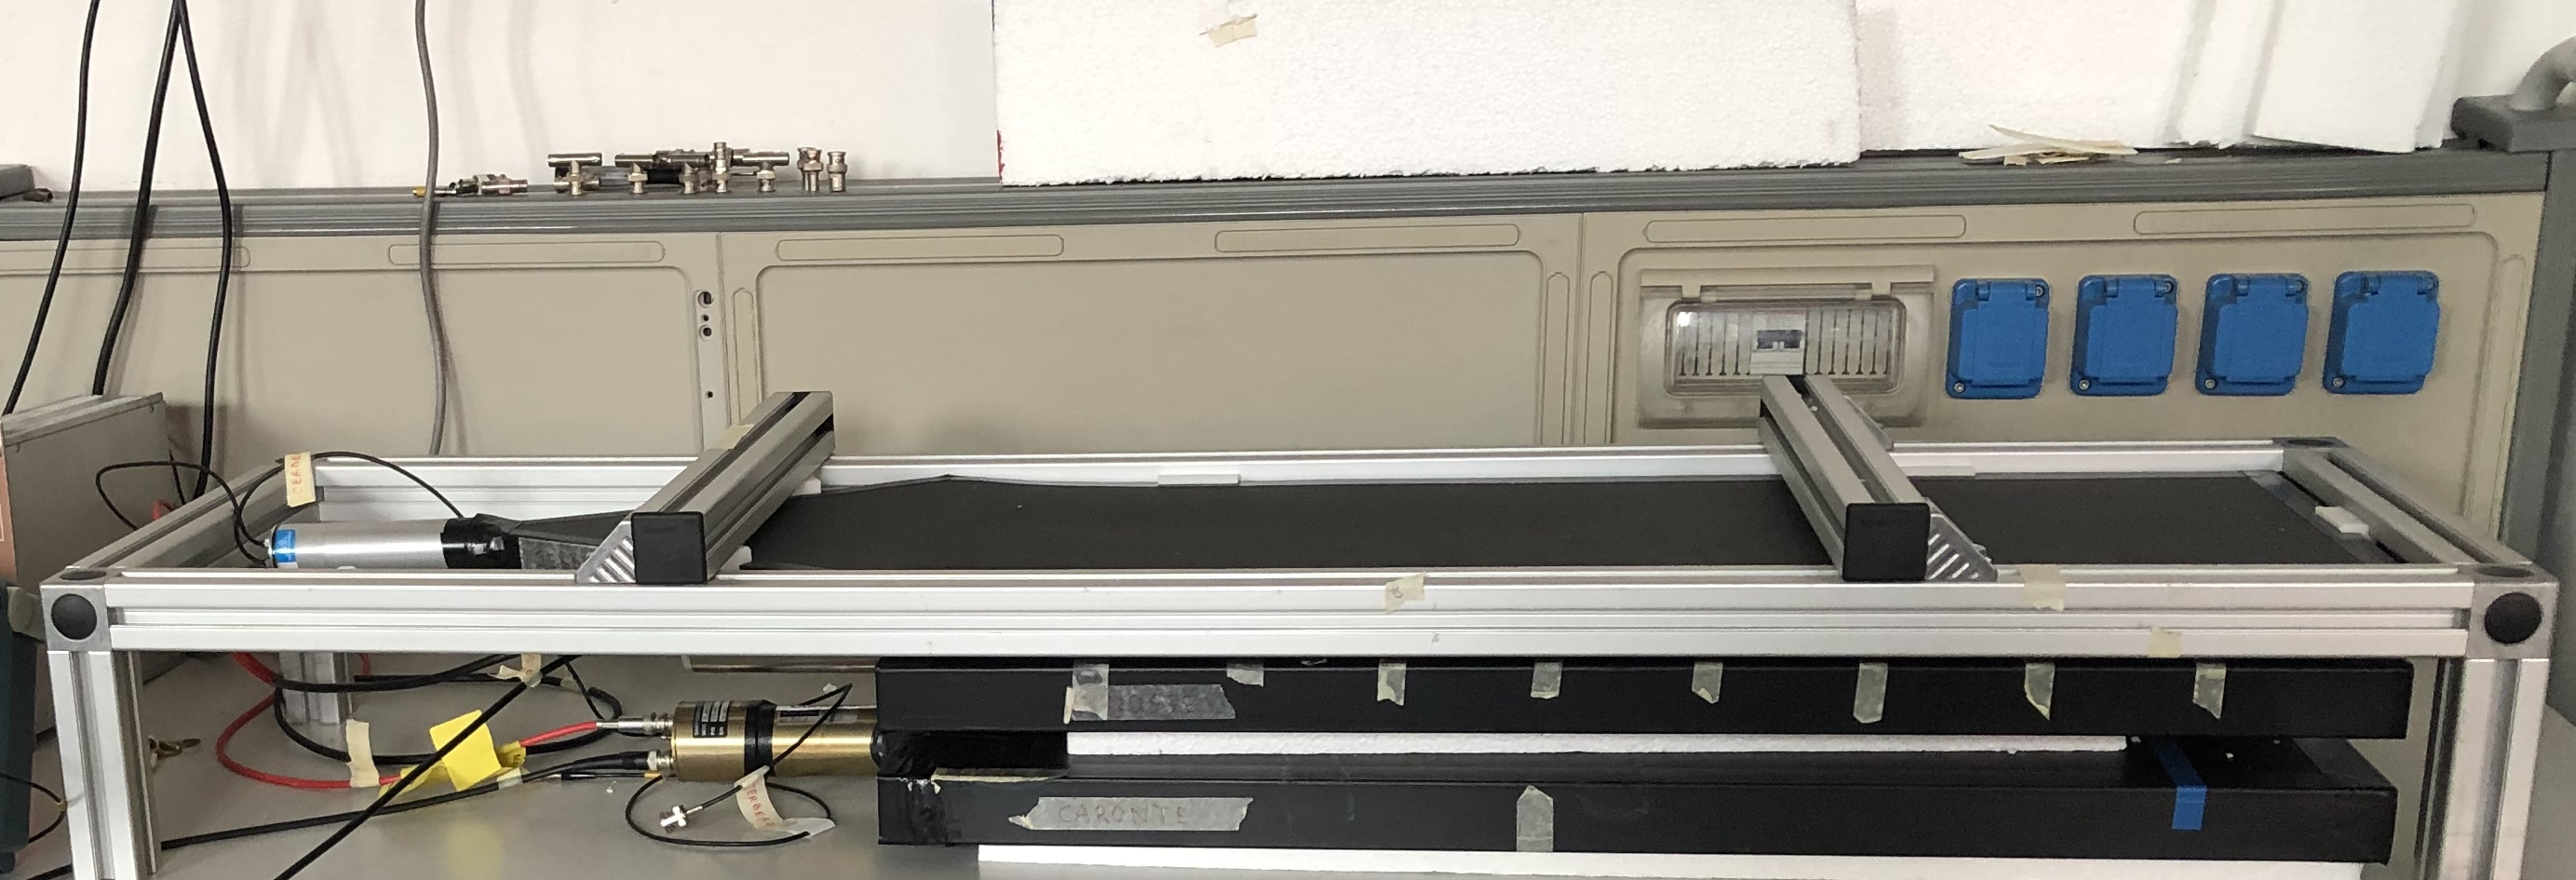
\includegraphics[width=\linewidth]{riv}
	\caption{Plastic scintillators.}
	\label{rivelatori}
\end{figure}

\subsection{Electronic instrumentation } \label{Electronic instrumentation}

The electronic instrumentation used during the whole experiment is:
\begin{itemize}
	\item NIM Crate (CAEN)
	\item Quad Scaler And Preset Counter/Timer N1145 (CAEN)
	\item Programmable Logic Unit N81 (CAEN)
	\item NIM Model 622 Quad 2-Fold Logic Unit(LeCroy)
	\item Dual Delay Unit N108 (CAEN)
	\item Dual Timer N93 (CAEN)
	\item Logic FAN-IN FAN-OUT N454 (CAEN)
	\item Discriminator N417 (CAEN)
	\item 2CH High Voltage Power Supply N1495 (CAEN)
	\item High Voltage Power Supply N556 (ORTEC)
	\item Desktop Digitizer (CAEN)
\end{itemize}